\documentclass[a4paper]{article}

% Import some useful packages
\usepackage[margin=0.5in]{geometry} % narrow margins
\usepackage[utf8]{inputenc}
\usepackage[english]{babel}
\usepackage{hyperref}
\usepackage{minted}
\usepackage{amsmath}
\usepackage{xcolor}
\usepackage{graphicx}
\definecolor{LightGray}{gray}{0.95}

\title{Peer-review of INF3/4331 assignment 5}

\begin{document}
\maketitle

\section{Introduction}

Well done on finishing assignment 5!
The peer-review for this assignment will be slightly different to the previous ones and  will reflect how professional software development is actually performed today. Specifically, in collaborative software development one does typically not write \LaTeX reviews to suggest code improvements.  

Consider the following example. Sarah owns a project repository and Bill would like to suggest an improvement or new feature to that project. The procedure for Bill's code contribution consists of five steps:
\begin{enumerate}
\item Bill creates a \emph{copy} of Sarah's repository. This copy is called a `fork'.
\item Bill implements his improvements or new feature and pushes these changes to his `fork'.
\item Bill send a request to Sarah to include his changes. He does this by creating a `pull request'.
\item Sarah reviews Bill's changes and can either reject or accept the pull request. If rejected, Bill can commit further improvement to his fork until Sarah is happy.
\item Once the pull request is accepted, Sarah merges the pull request. This means that Bill's code changes will be merged inot Sarah's code repository.
\end{enumerate}

The figure below visualizes these steps. Note that this procedure even works if Bill does not have write access to Sarah's repository.

\begin{figure}[h!]
\centering
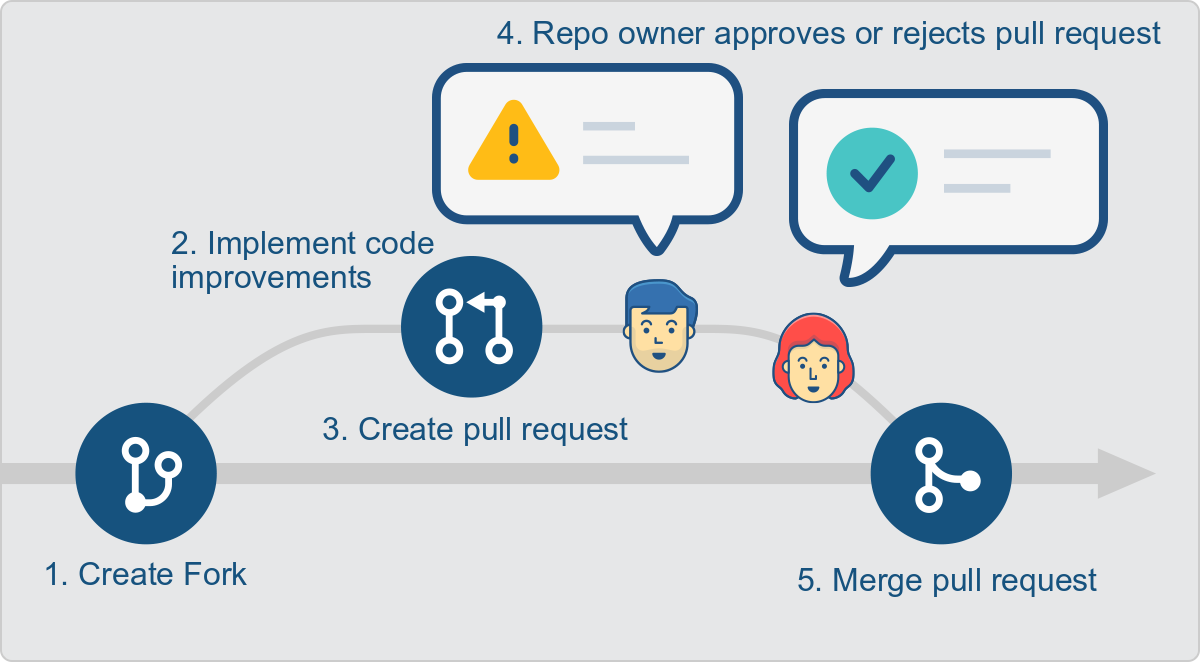
\includegraphics[width=0.8\textwidth]{collaboration.png}
\caption{Steps of modern collaborative software development}\label{fig:steps}
\end{figure}


\subsection{Goal}
In this peer-review we will perform steps 1-3 of the steps described in Figure \ref{fig:steps}.
That is, you will create a \emph{copy} of the repo (a `fork') and implement your improvements directly to the code. Once finished, you will request to include your improvements into the students original repo (a `pull request'). This `fork-then-pull-request' is a very common practice in professional code development. 

The spirit of the ``review'' is the same as before: \emph{make constructive changes} and use \emph{your knowledge and experience} to improve the solution. However, in contrast to the previous peer-review, this time you will actually implement code improvements. You will still be assigned to groups of 3, but it might be beneficial for each of you be responsible for one pull-request each. You should help each other in the group to improve each other pull requests as much as possible, but you will only be graded for your own pull request. 

The following list guides you through this process:
\begin{enumerate}
\item Visit the repository URL that you need to review, i.e. something like \\ \url{https://github.com/UiO-INF3331/INF3331-UiOUser}.
\item Click on the `Fork' button on the top right to create your personal copy of the repository. 
\\
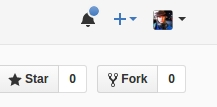
\includegraphics[width=0.2\textwidth]{Selection_001}
\item Once forked, you will be forwarded to the repository page of your personal copy.
\\
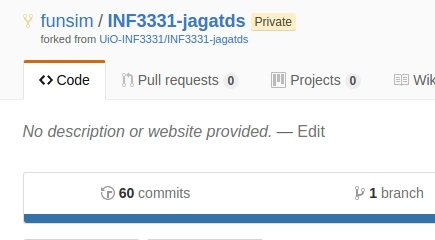
\includegraphics[width=0.2\textwidth]{Selection_003}
\item Clone this repository as usual to your computer.
\\
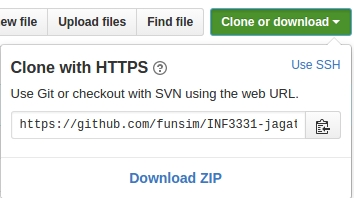
\includegraphics[width=0.2\textwidth]{Selection_005}
\item Review the code and implement improvements where possible. Commit and push these changes to your forked repository. Follow the guidelines in section \ref{sec:general_review} as a guideline. In case the student did not implement an assignment, you can skip the review of that assignment. 
\\
\item Once you are finished and committed the improvements, it is time to create a `pull request'. This will notify the reviewed student that you would like to apply your changes to the student's code base. You create the peer-review by visiting your for repository (i.e. \url{https://github.com/YourGithubUsername/INF3331-UiOUser}) and clicking on `New pull request':
\\
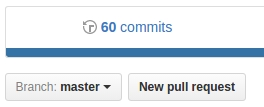
\includegraphics[width=0.2\textwidth]{Selection_006}
\\
In the description of the pull-request you should summarize and motivate the changes that you have made, as well as insert comments for specific parts of the code.
\end{enumerate}


More information about pull requests can be found on \url{https://help.github.com/articles/about-pull-requests}.


\subsection{Guidelines}\label{sec:general_review}
For each (coding) exercise, you should try to address and implement improvements to the following points:

\begin{itemize}
  \item Add docstrings where missing and where appropriate.
  \item Is the code working as expected? For non-internal functions (in particular for scripts that are run from the command-line), does the program handle invalid inputs sensibly? Can you make the code more reliable?
  \item Is part of the code unreadible or difficult to understand? Simplify the code, add comments where required, and use classes/functions to avoid duplicate code. 
\item Do \textbf{not} commit suggestions on how to improve code quality to the code - instead actually implement these changes. 
\end{itemize}

\textbf{Again:  you should \underline{implement improvements} in a pull-request and not just add suggestions into the code)!}
\bibliographystyle{plain}
\bibliography{literature}

\end{document}